\subsubsection{Polymethylmethacrylat}
\label{subsec:pofpmma}

Polymethylmethacrylat (PMMA) wurde erstmals 1928 von Otto Röhm hergestellt. Fünf
Jahre später wurde PMMA unter dem Namen
Plexiglas\textsuperscript{\textregistered} vermarktet. Wegen der hohen optischen
Durchlässigkeit und des geringen Gewichts eignet sich PMMA für den Einsatz in
der Automobilindustrie. Diese Eigenschaften sind ebenfalls ein Grund für die
Verwendung von PMMA in polymer optischen Fasern. \cite{pofwuppmma}

\paragraph{Polymerisation von Polymethylmethacrylat} Die Synthese von PMMA
erfolgt mittels einer radikalischen Polymerisation. Dabei wird zu dem Monomer
Methylmethacrylat (MMA) ein Radikalbildner hinzugefügt. Der Radikalbildner
zerfällt durch Licht- / Wärmezufuhr in Radikale. Diese lagern sich an die
C-C-Doppelbindung der Monomere an. Dadurch wird die Doppelbindung aufgespaltet
und das aktive Zentrum weitergegeben. Dieser Vorgang erzeugt wieder ein Radikal,
welches ebenfalls ein Methylmethacrylat angreift. Somit wächst die Monomerkette
zu einem Polymer an. Der Abbruch des Kettenwachstums kann entweder durch einen
Zusammenschluss mit einem weiteren Radikal oder durch eine Disproportionierung
geschehen. Beide Reaktionen haben eine Sättigung des aktiven Zentrums zur Folge.
\autoref{rec:pmma} fasst den Reaktionsablauf zusammen und zeigt, dass es sich
bei Polymethylmethacrylat um ein lineares Makromolekül, also um einen
Thermoplasten handelt.

\ifthenelse{\boolean{showPics}}{
    \begin{figure}[H]
        \begin{center}
            \footnotesize
            \setatomsep{1.7em}

            \chemnameinit{\chemfig{-[@{op,0.5}]CH_2-C(-[2]CH_3)(-[6]C(=[:-150]\lewis{36,O})(-[:-30]\lewis{57,O}-[:30]CH_3))-[@{cl,0.9},3.1pt]}}

            \chemname{\chemfig{R-R}}{\\\\Radikalbildner}
            \chemsign{+ $\scriptstyle n$}
            \chemname{\chemfig{H_2C=C(-[:60]CH_3)(-[:-60]C(=[:-120]\lewis{46,O})(-\lewis{26,O}-CH_3))}}{\\\\Methylmethacrylat}
            \chemrel{->}
            \chemname{\chemfig{-[@{op,0.5}]CH_2-C(-[2]CH_3)(-[6]C(=[:-150]\lewis{36,O})(-[:-30]\lewis{57,O}-[:30]CH_3))-[@{cl,0.9},3.1pt]}}{\\\\Polymethylmethacrylat}
            \makebraces[20pt,35pt]{n}{op}{cl}

            \caption{radikalische Polymerisation von Polymethylmethacrylat}
            \label{rec:pmma}
        \end{center}
    \end{figure}
}{}

\paragraph{Herstellung von Polymethylmethacrylat}

Der folgende Versuch zeigt die Herstellung von PMMA mit den Radikalbildner
Azodiisobutyronitril und Dibenzoylperoxid. \\

\par

Material:
\begin{compactitem}
    \item Heizplatte, Reagenzgläser, Thermometer, Wasserbad, Spatel, Waage, Stativ
    \item Chemikalien: \\[5pt]
    \begin{tabular}{ll}
    Methylmethacrylat (MMA): & Sicherheitshinweis CAS Nr. 80-62-1 \\
    & (entzündlicher und reizender Stoff) \\
    Azodiisobutyronitril (AIBN): & Sicherheitshinweis CAS Nr. 78-67-1 \\
    & (entzündlicher und reizender Stoff) \\
    Dibenzoylperoxid (BPO): & Sicherheitshinweis CAS Nr. 94-36-0 \\
    & (entzündlicher, reizender und explosiver Stoff)
    \end{tabular}
\end{compactitem}~\par

\\Schutzvorkehrungen:
\begin{compactitem}
    \item Abzug, Schutzkleidung, Handschuhe, Schutzbrille
\end{compactitem}~\par

\\Versuchsablauf \cite{pofversuch}:
\begin{compactenum}
    \item Das Wasserbad wird unter dem Abzug auf ca. 70°C erhitzt.
    \item In einem Reagenzglas werden 5 ml MMA mit 50 mg des Radikalbildners AIBN oder BPO vermischt.
    \item Das Reagenzglas wird im Wasserbad erhitzt (siehe \autoref{fig:mmawasserbad}).
    \item Sobald der Inhalt des Reagenzglases zähflüssig ist, wird das Reagenzglas aus dem Wasserbad genommen.
    \item Nachdem die Polymerisation abgeschlossen ist, wird das Reagenzglas zerschlagen und das PMMA entnommen.
\end{compactenum}

\ifthenelse{\boolean{showPics}}{
    \begin{figure}[h]
        \begin{center}
            \begin{minipage}[t]{0.3\textwidth}
                \begin{center}
                    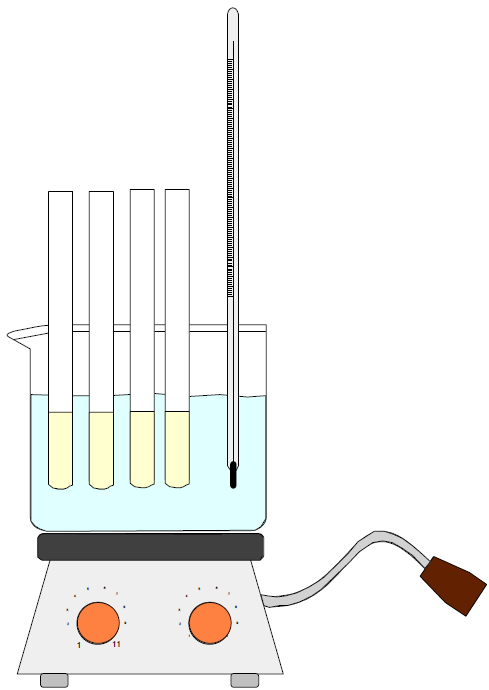
\includegraphics[height=0.1\textheight]{Bilder/Optische_Wellenleiter_Die_Polymer_Optische_Faser/Kernmaterialien/mmawasserbad.png}
                    \caption[Versuchsaufbau]{Versuchsaufbau}
                    \label{fig:mmawasserbad}
                \end{center}
            \end{minipage}
            \hspace{0.025\textwidth}
            \begin{minipage}[t]{0.3\textwidth}
                \begin{center}
                    \includegraphics[height=0.1\textheight]{Bilder/Optische_Wellenleiter_Die_Polymer_Optische_Faser/Kernmaterialien/pmmastuecke.png}
                    \caption[PMMA-Stücke]{PMMA-Stücke}
                    \label{fig:pmmastuecke}
                \end{center}
            \end{minipage}
            \hspace{0.025\textwidth}
            \begin{minipage}[t]{0.3\textwidth}
                \begin{center}
                    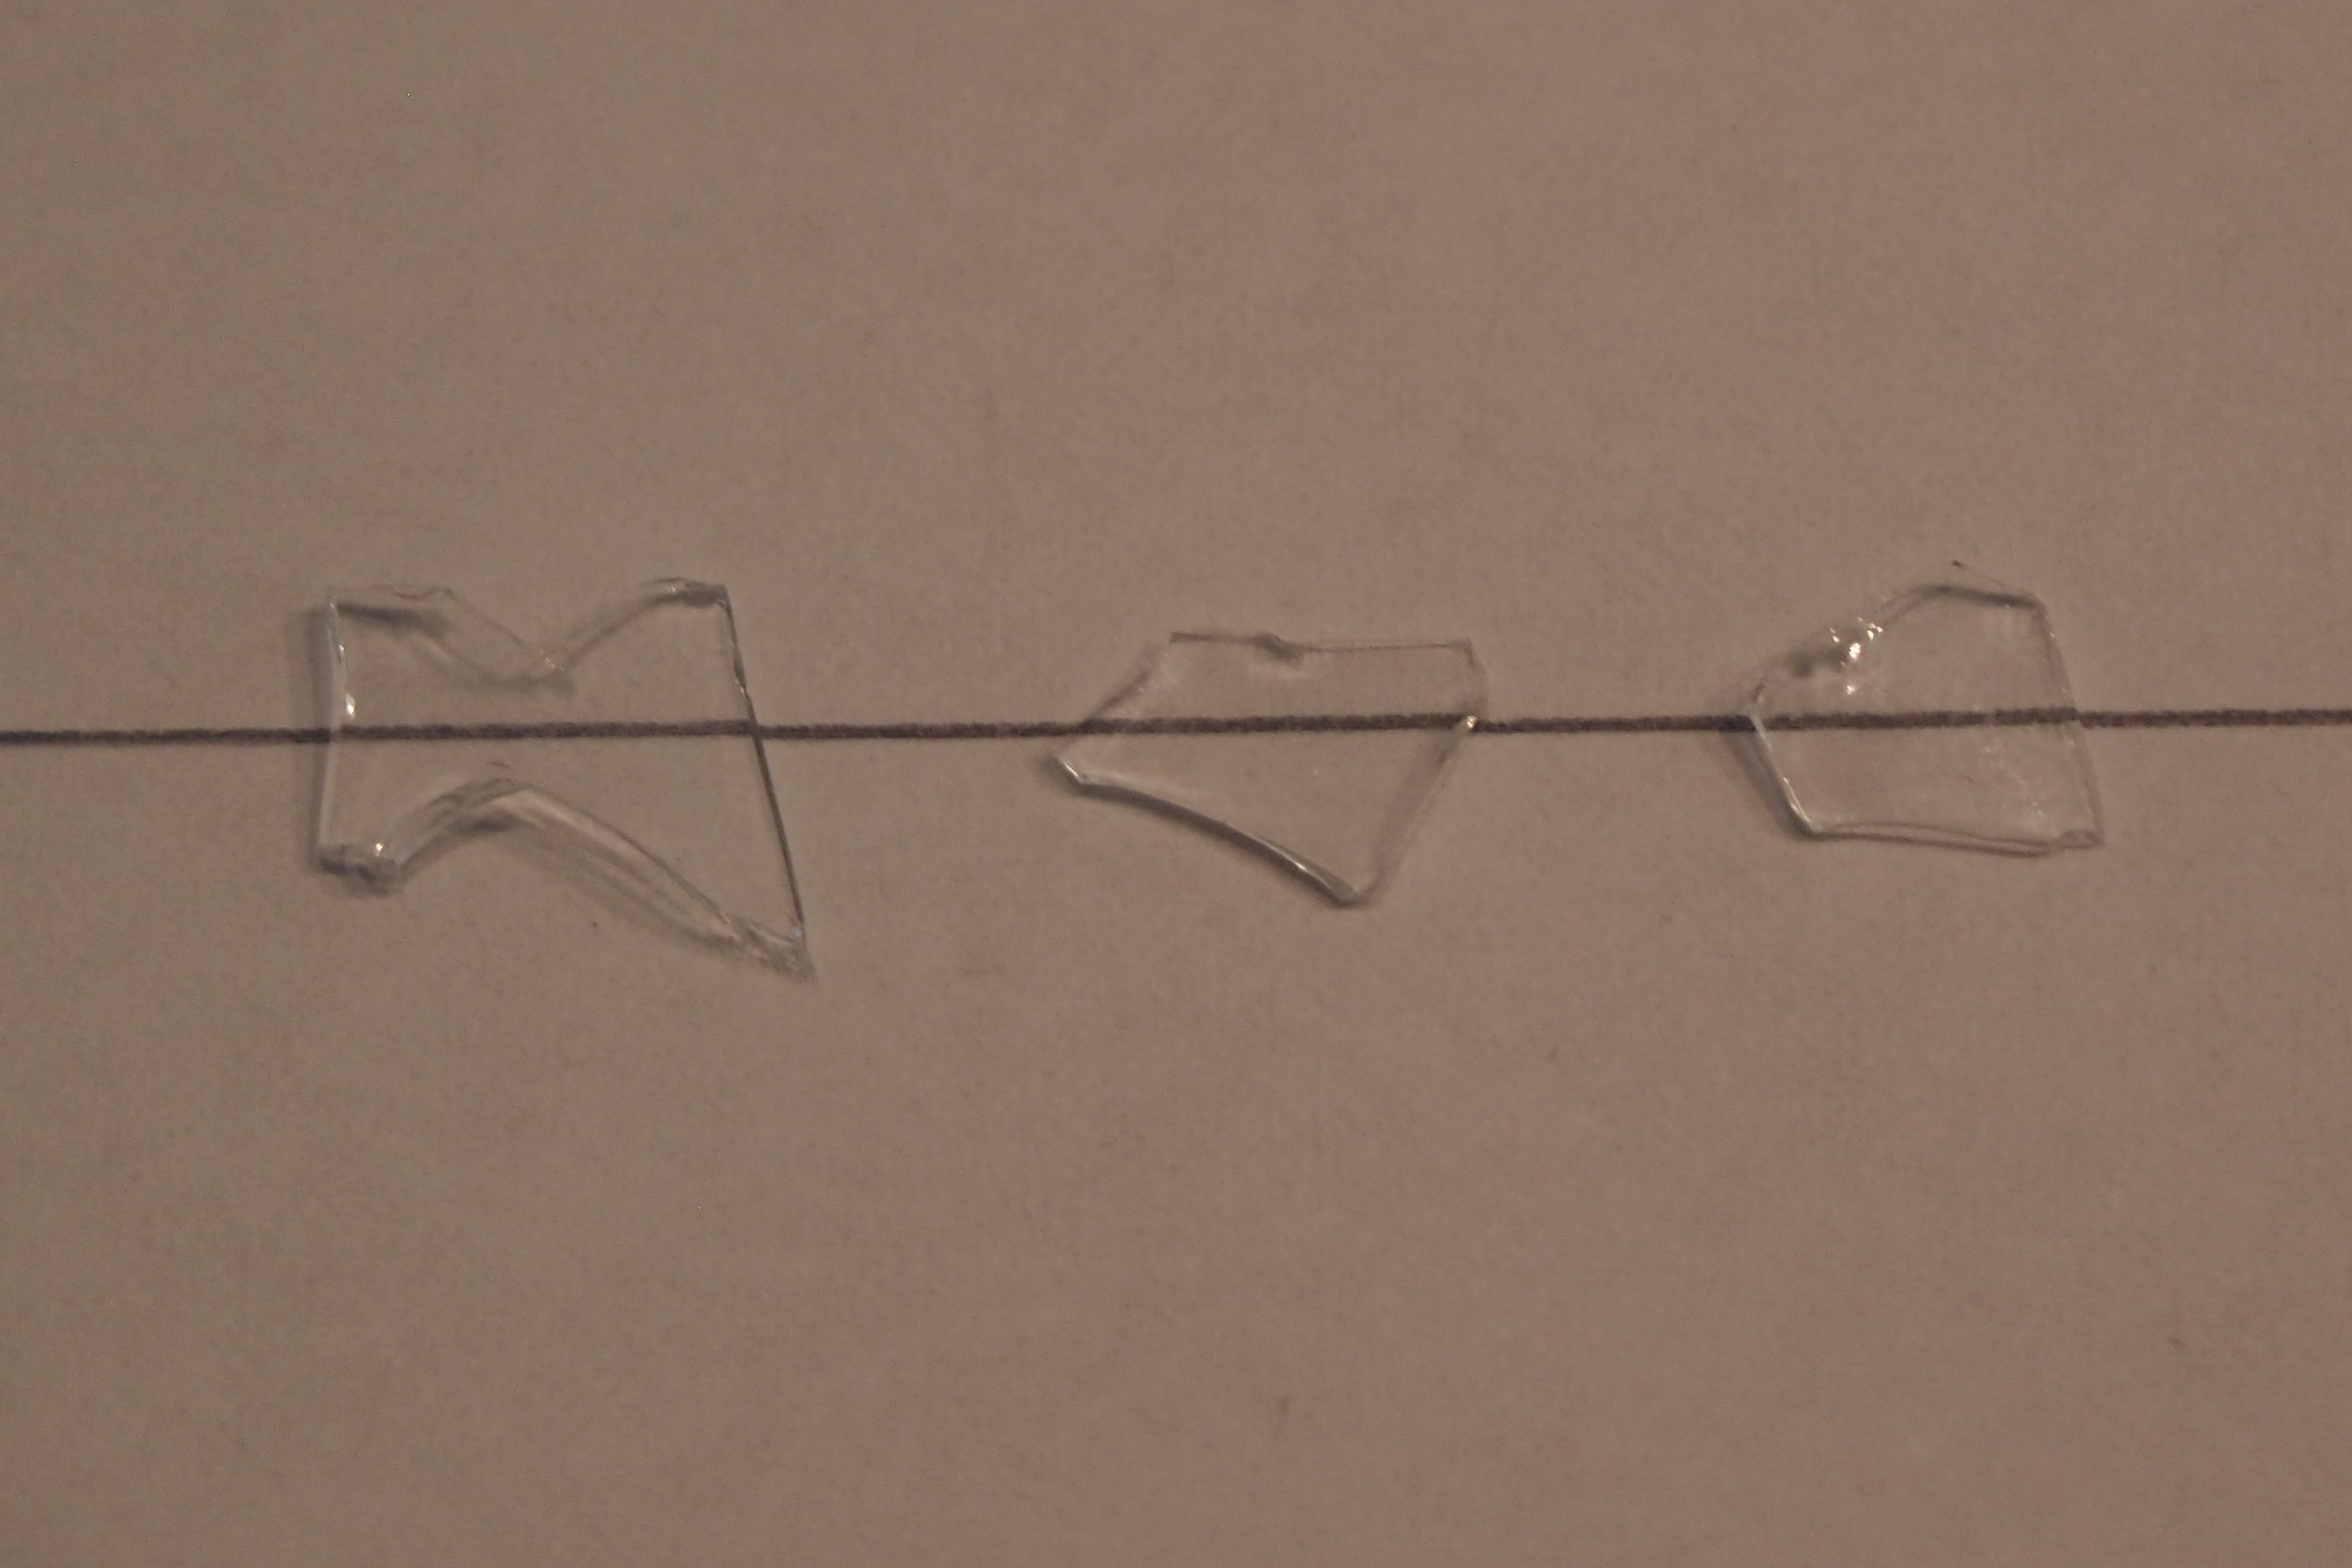
\includegraphics[height=0.1\textheight]{Bilder/Optische_Wellenleiter_Die_Polymer_Optische_Faser/Kernmaterialien/pmmaschnipsel.png}
                    \caption[PMMA-Schnipsel]{PMMA-Schnipsel}
                    \label{fig:pmmaschnipsel}
                \end{center}
            \end{minipage}
        \end{center}
    \end{figure}
}{}

Ergebnis: Die entstandenen PMMA-Stücke in \autoref{fig:pmmastuecke} haben eine
geringe Qualität, da Luftblasen in dem Kunststoff eingeschlossen sind. Außerdem
ist eine gelbliche Färbung erkennbar, die von dem unverbrauchten Radikalbildner
AIBN verursacht wird. Dieser wurde in den beiden linken Stücken eingesetzt. In
kleinen Stücken lässt sich die hohe optische Durchlässigkeit von PMMA erkennen.
Der Strich in \autoref{fig:pmmaschnipsel} unter den kleinen PMMA-Stücken ist
sehr gut sichtbar und wird nur geringfügig verschoben. Der Versuch zeigt auch,
dass PMMA relativ einfach herzustellen ist.
